\section{Технический проект}
\subsection{Общая характеристика организации решения задачи}

Задача заключается в создании веб-приложения для диагностики заболеваний томатов и выдачи рекомендаций по их лечению и профилактике. Приложение поможет агрономам и дачникам быстро выявлять болезни растений и принимать меры для сохранения урожая.

Приложение представляет собой веб-страницу, доступную через Интернет по адресу, например, www.доменПриложения.ru. На странице размещены текстовые описания, поле для загрузки изображений и область для вывода результатов анализа.

\subsection{Обоснование выбора технологии проектирования}

Для создания приложения выбраны технологии, которые обеспечивают высокую производительность, удобство для пользователей и простоту интеграции с моделью машинного обучения.

\subsubsection{Язык программирования Python}

Python -- высокоуровневый язык программирования с динамической типизацией. Его интерпретатор позволяет запускать код на различных платформах, включая Windows, macOS и Linux, без необходимости компиляции. Официальная документация поддерживает разные подходы к программированию, включая процедурный, объектно-ориентированный и функциональный стили, что даёт разработчикам гибкость\cite{python2} \cite{python3}. 

В 2025 году Python остаётся одним из самых популярных языков благодаря своему простому синтаксису и большому количеству  библиотек, которые и позволяют создавать на нём веб-приложения и модели ИИ \cite{python4}\cite{python1}.

\subsubsection{Фреймворк PyTorch}

PyTorch -- это инструмент, созданный для работы с нейронными сетями на Python. Он используется разработчиками, когда нужно быстро протестировать идею и собрать прототип, особенно в проектах, связанных с машинным обучением. Его ценят за гибкость, читаемость кода и большое количество готовых решений.

Открытый исходный код PyTorch позволяет любому разработчику внести изменения или адаптировать его под собственные задачи. Благодаря этому вокруг проекта сформировалось большое и активное сообщество. Постоянно появляются новые библиотеки, расширения и обучающие материалы, которые делают работу с фреймворком ещё проще \cite{yolo6}.

Среди особенностей -- поддержка как классических, так и продвинутых архитектур нейросетей. Встроенные модули позволяют обрабатывать данные, визуализировать результаты и отслеживать, как ведёт себя модель во время обучения.

Благодаря всему этому PyTorch активно применяется в разных сферах.

\subsubsection{YOLO}

YOLOv11 -- это одна из последних разработок в серии алгоритмов для распознавания объектов на изображениях. Эту версию представила команда Ultralytics. Данная модель стала логичным продолжением предыдущих модификаций YOLO, сохранив при этом основной подход: находить и определять объекты за один проход по изображению \cite{yolo8}.

Главное, за что ценят YOLO -- это скорость и точность. Она справляется с обработкой видео и изображений практически в реальном времени. Такая производительность достигается благодаря улучшенной архитектуре сверточной нейросети и доработанному механизму обучения. Разработчики также внедрили более точные методы предобработки данных, что заметно повысило стабильность работы модели \cite{yolo2}. 

Для обучения YOLO требуется датасет, где каждый объект уже размечен. После обучения модель может точно распознавать объекты даже на тех изображениях, которых не было в тренировочном наборе. Например, её можно применять для поиска признаков заболеваний на листьях растений — она определит поражённые участки по загруженному фото \cite{yolo1}.

На графике ~\ref{graf:image} ниже представлены результаты сравнения 11-ой версии с предшествующими ей. 
\begin{figure}[H]
	\centering
	\includegraphics[width=1\linewidth]{garfYolo.png}
	\caption{График сравнения версий YOLO}
	\label{graf:image}
\end{figure}

По графику видно, что модель демонстрирует высокую точность на наборе данных COCO, достигая значения около 54.5, при меньшей задержке по времени в сравнении с другими моделями \cite{yolo7}.

Архитектура YOLOv11 делится на три основные части: Backbone, Neck и Head. Они представлена на схеме ~\ref{йоло:image}.

\begin{figure}[H]
	\includegraphics[width=1\linewidth, height=1.2\linewidth]{yolo.jpg}
	\caption{Архитектура YOLO 11}
	\label{йоло:image}
\end{figure}

\paragraph{Backbone}

Backbone анализирует входное изображение размером 640x640 пикселей. Основной его задачей является выделение важных деталей, таких как края, текстуры или пятна на листе. Backbone состоит из нескольких слоёв, которые постепенно уменьшают размер изображения и извлекают признаки \cite{yolo8}:

\begin{enumerate}
	\item Свёрточные слои отвечают за процесс свёртки, при котором фильтр проходит по изображению и выделяет его особенности. В YOLO11 такие слои уменьшают размер изображения шаг за шагом: сначала до 320x320, потом до 160x160, 80x80, 40x40 и 20x20. На каждом этапе детали становятся более обобщёнными.
	
	\item Блоки C3K2 представляют собой улучшенную версию блоков C3, которые использовались в более ранних моделях YOLO. Такой блок включает несколько свёрток и остаточные связи. Остаточные связи позволяют пропустить часть данных через блок без изменения и добавить их к результату. Это помогает модели бороться с проблемой затухающего градиента, когда верхние слои практически не обучаются при малом значении градиента во время обратного распространения. Эти блоки применяются на разных этапах backbone, чтобы выделить признаки разного уровня.
	
	\item C2PSA (Cross-Stage Partial Self-Attention) -- это технология срабатывает на этапе уменьшения размерности до 20x20, в её основе лежит алгоритм само-внимания. Она помогает модели сосредоточиться на важных частях изображения, не отвлекаясь на второстепенные. Само-внимание смотрит, как разные части изображения связаны между собой, что полезно для обнаружения мелких деталей.
\end{enumerate}

Backbone формирует карты признаков и передаёт их в neck.

\paragraph{Neck}

Neck собирает данные из backbone и готовит их к финальному этапу детекции. Эта часть объед
иняет информацию с разных масштабов, чтобы модель могла лучше находить мелкие объекты. Neck состоит из следующих модулей \cite{yolo3}:

\begin{enumerate}
	\item SPFF (Spatial Pyramid Pooling Fast) -- это модуль, который улучшает стандартный SPP из прошлых версий YOLO. SPP берёт карту признаков, и применяет пулинг с разными размерами фильтров, чтобы выделить признаки разной детализации \cite{yolo4}. Пулинг — это процесс, который берёт, например, максимальное значение в окне 2x2, уменьшает размер карты, но сохраняет важные данные. SPFF делает это быстрее за счёт особых свёрток, что экономит время без потери качества.
	
	\item Слои Concat соединяют карты признаков разных размеров — 80x80, 40x40, 20x20, чтобы модель могла использовать данные с разных уровней.
	
	\item Upsample увеличивает размер карты признаков. Этот слой использует интерполяцию, добавляя промежуточные значения, чтобы «растянуть» данные. Это нужно, чтобы мелкие детали можно было передать на более крупные масштабы и соединить с другими признаками через Concat.
	
	\item Блоки C3K2 используются в neck, чтобы ускорить работу. Они продолжают выделять признаки, но требуют меньше вычислений, что важно для увеличения скорости обработки.
	
\end{enumerate}

Neck готовит три карты признаков размерностями 80x80, 40x40, 20x20 и отправляет их в head.

\paragraph{Head}

Head -- это последняя часть модели, которая выдаёт результаты на основе данных из Neck. Она определяет координаты рамок, классы и вероятность в трёх масштабах.

\begin{enumerate}
	\item Блок Detect обрабатывает каждый масштаб и делает предсказания координат рамок, вероятностей классов и уверенности. Он использует свёртки, чтобы получить эти данные.
	
	\item Dual Label Assignment -- это новый способ, который YOLO11 использует для работы с метками. Обычно модели детекции привязывают одну рамку к одному объекту, но в реальных данных объекты могут пересекаться. Данная технология позволяет модели рассматривать несколько вариантов меток для одного объекта, что делает её точнее в сложных случаях.
	
\end{enumerate}

Head выдаёт итоговые данные, которые приложение использует для показа результатов.

\paragraph{Применение в задаче}

В проекте диагностики заболеваний томатов YOLO11 берёт изображение листа размером 640x640. Backbone выделяет признаки, такие как текстура и пятна, с помощью свёрток и C3K2, а C2PSA помогает найти мелкие детали. Neck соединяет эти признаки через SPFF и Concat, чтобы учесть разные масштабы. Head выдаёт результаты, определяя, есть ли болезнь. YOLO11 подходит для этой задачи, так как он быстро работает, точно определяет мелкие объекты и хорошо справляется с анализом изображений растений в реальном времени \cite{yolo10}.

\subsubsection{Фреймворк Flask}

Flask -- это легковесный веб-фреймворк на языке Python, который часто используют для разработки простых и понятных веб-приложений. Он не навязывает структуру проекта, поэтому подойдёт как новичкам, так и разработчикам, которым нужен контроль над архитектурой \cite{flask1}.

В отличие от более тяжёлых решений, Flask не включает в себя избыточных модулей. Вместо этого он предлагает только базовые инструменты -- маршрутизацию, работу с запросами и шаблонизатор \cite{flask2}.

Для разработки веб-интерфейса системы распознавания заболеваний растений Flask подойдёт особенно хорошо. Он позволяет быстро реализовать обработку изображений, вывод результатов и взаимодействие с нейросетью. Благодаря простому синтаксису и большому количеству обучающей информации, с реализацией приложений не возникает серьёзных трудностей, даже при ограниченном опыте в веб-программировании \cite{flask4}.

Фреймворк хорошо работает на любых операционных системах и легко разворачивается как на локальной машине, так и на сервере. Это делает Flask удобным выбором для небольших и средних проектов \cite{flask5}.

\subsection{Диаграмма компонентов}

 На рисунке \ref{comp:image} изображена диаграмма компонентов системы.
 
 \begin{figure}[ht]
 	\center{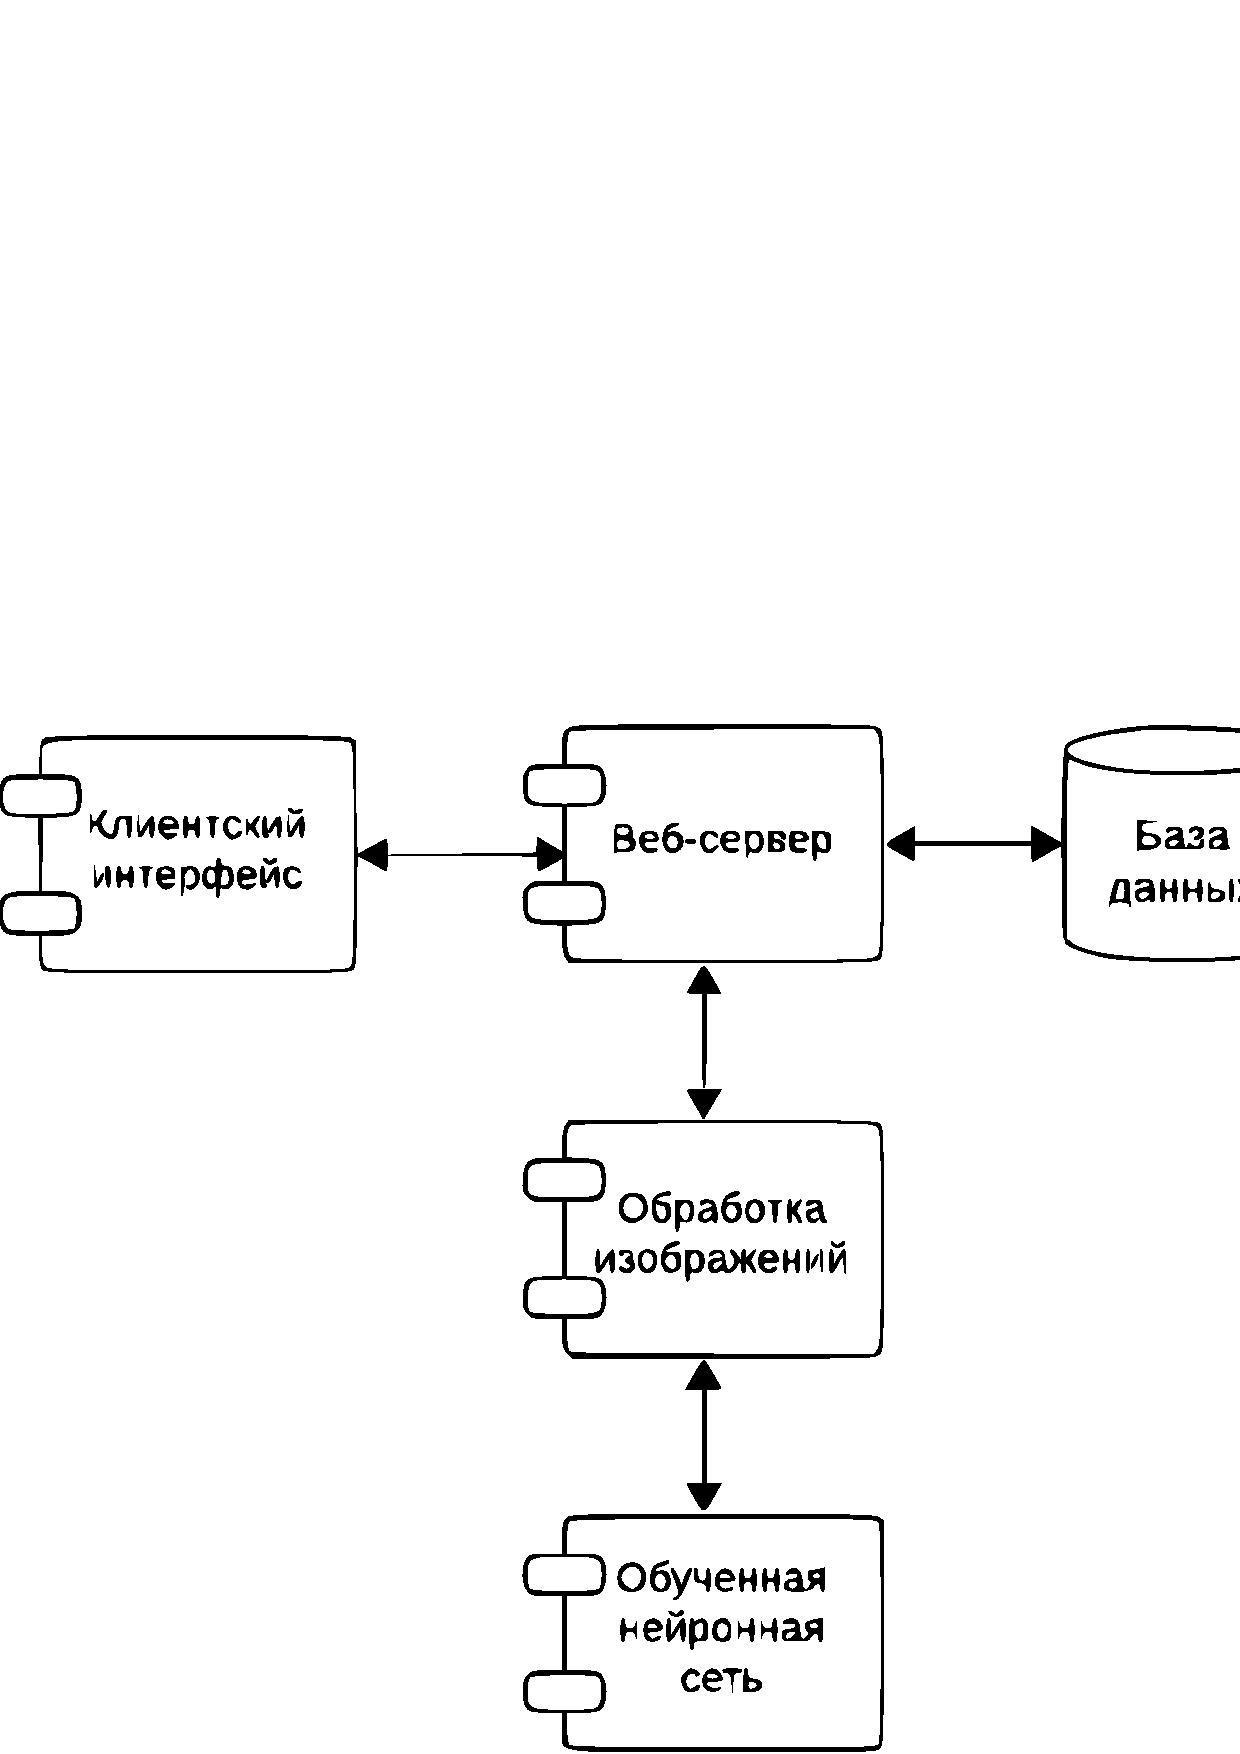
\includegraphics[width=1\linewidth]{Диаграмма компонентов.png}}
 	\caption{Диаграмма компонентов}
 	\label{comp:image}
 \end{figure}
 
 Диаграмма показывает, как устроено веб-приложение для диагностики заболеваний томатов. Она представлена в виде схемы с пятью основными блоками, соединёнными стрелками. Они указывают, как данные передаются между частями приложения. Каждая часть выполняет свою задачу, чтобы обеспечить работу системы.
 
 Клиентский интерфейс -- это веб-страница, через которую пользователь загружает изображение листьев. На этой же странице он видит результат анализа.%: найденный недуг, советы по его устранению и методы для профилактики.
 
 Веб-сервер стоит в центре схемы и управляет всем процессом. Он принимает запросы от интерфейса, направляет данные в нужные модули и возвращает результат пользователю. 
 
 База данных хранит описание болезней томатов, методы лечения, способы профилактики. Сервер обращается к ней, если модель нашла недуг.
 
 Модуль обработки изображений подготавливает загруженное фото для анализа. Он изменяет размер изображения, повышает резкость и контраст, а затем передаёт его в модель. 
 
 Нейронная сеть анализирует изображение и определяет, есть ли на фото болезнь и возвращает на сервер результат.

\subsection{Структура базы данных}

Сущности и отношения между ними отображены на ER-диаграмме.

 \begin{figure}[ht]
	\center{\includegraphics[width=1\linewidth]{диплом.png}}
	\caption{ER-диаграмма}
	\label{er:image}
\end{figure}


\begin{xltabular}{\textwidth}{|l|l|p{1.7cm}|X|}
	\caption{Атрибуты сущности diseases\label{diseases:table}}\\ \hline
	\centrow Поле & \centrow Тип & \centrow Обяза\-тельное & \centrow Описание \\ \hline
	\thead{1} & \thead{2} & \centrow 3 & \centrow 4 \\ \hline
	\endfirsthead
	\caption*{Продолжение таблицы \ref{diseases:table}} \\ \hline
	\thead{1} & \thead{2} & \centrow 3 & \centrow 4 \\ \hline
	\finishhead
	id & serial & true & Первичный ключт \\ \hline
	name & varchar(100) & true & Название болезни \\ \hline
	description & text & false & Подробное описание болезни \\ \hline
	affected\_parts & varchar(255) & false & Части растения, поражаемые болезнью \\ \hline
	environmental\_factors & text & false & Экологические факторы, способствующие болезни \\ \hline
	created\_at & timestamp & false & Дата и время создания записи \\ \hline
\end{xltabular}

\begin{xltabular}{\textwidth}{|l|l|p{1.7cm}|X|}
	\caption{Атрибуты сущности treatments\label{treatments:table}}\\ \hline
	\centrow Поле & \centrow Тип & \centrow Обяза\-тельное & \centrow Описание \\ \hline
	\thead{1} & \thead{2} & \centrow 3 & \centrow 4 \\ \hline
	\endfirsthead
	\caption*{Продолжение таблицы \ref{treatments:table}} \\ \hline
	\thead{1} & \thead{2} & \centrow 3 & \centrow 4 \\ \hline
	\finishhead
	id & serial & true & Первичный ключ \\ \hline
	disease\_id & integer & true & Внешний ключ, ссылка на таблицу diseases \\ \hline
	treatment\_method & text & true & Описание методов лечения \\ \hline
\end{xltabular}

\begin{xltabular}{\textwidth}{|l|l|p{1.7cm}|X|}
	\caption{Атрибуты сущности preventions\label{preventions:table}}\\ \hline
	\centrow Поле & \centrow Тип & \centrow Обяза\-тельное & \centrow Описание \\ \hline
	\thead{1} & \thead{2} & \centrow 3 & \centrow 4 \\ \hline
	\endfirsthead
	\caption*{Продолжение таблицы \ref{preventions:table}} \\ \hline
	\thead{1} & \thead{2} & \centrow 3 & \centrow 4 \\ \hline
	\finishhead
	id & serial & true & Первичный ключ \\ \hline
	disease\_id & integer & true & Внешний ключ, ссылка на таблицу diseases \\ \hline
	prevention\_measure & text & true & Описание мер профилактики \\ \hline
\end{xltabular}

